\documentclass{article}
\usepackage[margin=15mm]{geometry}
\usepackage{pgfplots}
\pgfplotsset{compat=1.18}
\pagestyle{empty}
\begin{document}
% E10 means and sample standard deviations; successful runs only.
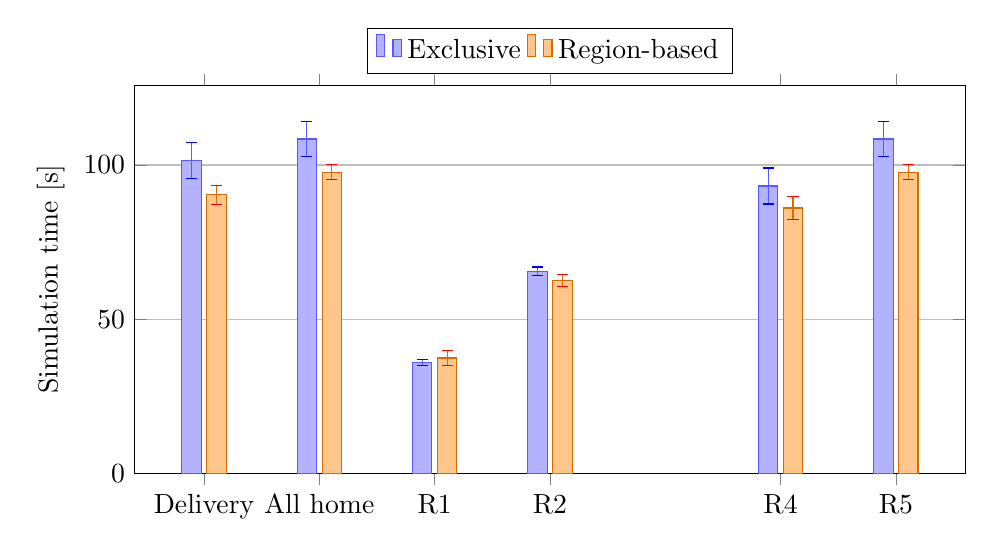
\begin{tikzpicture}
\begin{axis}[ybar,bar width=7pt,width=\linewidth,height=6.5cm,
symbolic x coords={Delivery,All home,R1,R2,R3,R4,R5},xtick=data,ymin=0,ylabel={Simulation time [s]},
legend style={at={(0.5,1.03)},anchor=south,legend columns=2},enlarge x limits=0.1,ymajorgrids=true]
\addplot+[draw=blue!65,fill=blue!30,error bars/.cd,y dir=both,y explicit] coordinates {(Delivery,101.4556) +- (0,5.8069) (All home,108.4444) +- (0,5.8040) (R1,35.8444) +- (0,0.9564) (R2,65.4833) +- (0,1.4420) (R4,93.1944) +- (0,5.8248) (R5,108.4444) +- (0,5.8040)};
\addlegendentry{Exclusive}
\addplot+[draw=orange!85!black,fill=orange!45,error bars/.cd,y dir=both,y explicit] coordinates {(Delivery,90.3722) +- (0,3.0656) (All home,97.6833) +- (0,2.4439) (R1,37.3722) +- (0,2.4223) (R2,62.4556) +- (0,1.9143) (R4,86.0556) +- (0,3.7234) (R5,97.6833) +- (0,2.4439)};
\addlegendentry{Region-based}
\end{axis}
\end{tikzpicture}
\clearpage
% Representative: lower median successful makespan in each mode. Bars are participation, NOT motion.
% exclusive, repetition 9
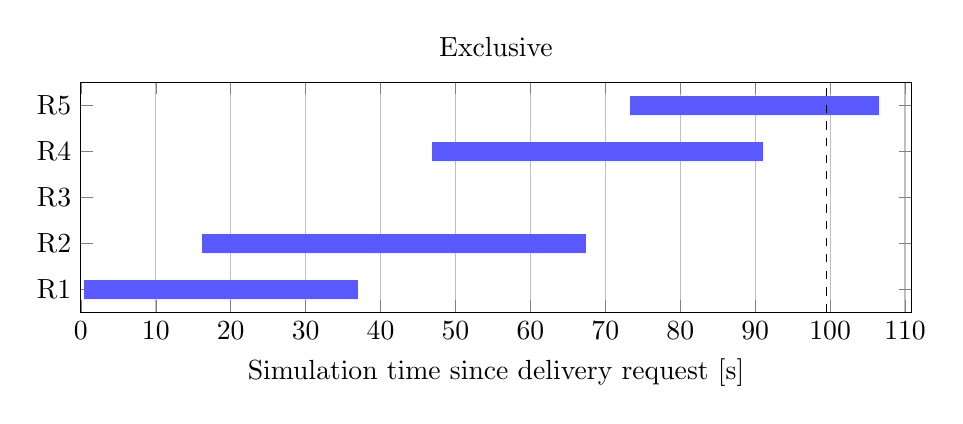
\begin{tikzpicture}
\begin{axis}[width=\linewidth,height=4.5cm,title={Exclusive},xmin=0,xmax=110.812,
ymin=0.5,ymax=5.5,ytick={1,2,3,4,5},yticklabels={R1,R2,R3,R4,R5},xlabel={Simulation time since delivery request [s]},xmajorgrids=true]
\addplot+[no marks,line width=7pt,blue!65] coordinates {(0.350,1) (37.050,1)};
\addplot+[no marks,line width=7pt,blue!65] coordinates {(16.150,2) (67.450,2)};
\addplot+[no marks,line width=7pt,blue!65] coordinates {(46.900,4) (91.100,4)};
\addplot+[no marks,line width=7pt,blue!65] coordinates {(73.300,5) (106.550,5)};
\addplot[black,dashed] coordinates {(99.550,0.5) (99.550,5.5)};
\end{axis}
\end{tikzpicture}\par
% region, repetition 10
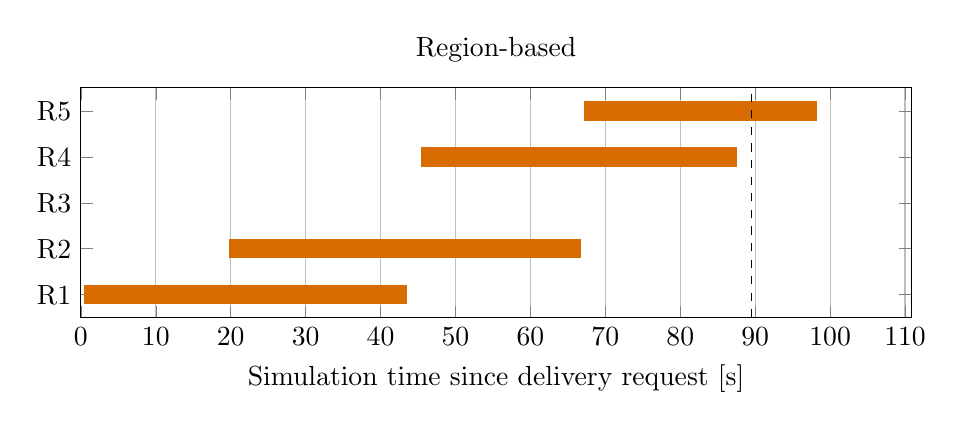
\begin{tikzpicture}
\begin{axis}[width=\linewidth,height=4.5cm,title={Region-based},xmin=0,xmax=110.812,
ymin=0.5,ymax=5.5,ytick={1,2,3,4,5},yticklabels={R1,R2,R3,R4,R5},xlabel={Simulation time since delivery request [s]},xmajorgrids=true]
\addplot+[no marks,line width=7pt,orange!85!black] coordinates {(0.400,1) (43.550,1)};
\addplot+[no marks,line width=7pt,orange!85!black] coordinates {(19.800,2) (66.700,2)};
\addplot+[no marks,line width=7pt,orange!85!black] coordinates {(45.350,4) (87.550,4)};
\addplot+[no marks,line width=7pt,orange!85!black] coordinates {(67.100,5) (98.250,5)};
\addplot[black,dashed] coordinates {(89.550,0.5) (89.550,5.5)};
\end{axis}
\end{tikzpicture}\par
\clearpage
% E10 means and sample standard deviations; successful runs only.
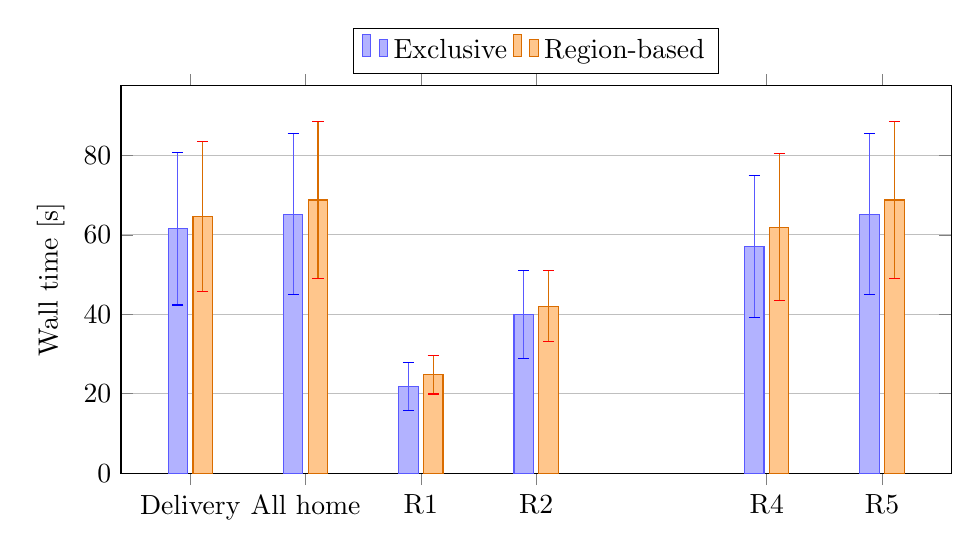
\begin{tikzpicture}
\begin{axis}[ybar,bar width=7pt,width=\linewidth,height=6.5cm,
symbolic x coords={Delivery,All home,R1,R2,R3,R4,R5},xtick=data,ymin=0,ylabel={Wall time [s]},
legend style={at={(0.5,1.03)},anchor=south,legend columns=2},enlarge x limits=0.1,ymajorgrids=true]
\addplot+[draw=blue!65,fill=blue!30,error bars/.cd,y dir=both,y explicit] coordinates {(Delivery,61.5734) +- (0,19.2392) (All home,65.1480) +- (0,20.2714) (R1,21.8063) +- (0,6.0977) (R2,39.9784) +- (0,11.1377) (R4,57.0611) +- (0,17.8428) (R5,65.1480) +- (0,20.2714)};
\addlegendentry{Exclusive}
\addplot+[draw=orange!85!black,fill=orange!45,error bars/.cd,y dir=both,y explicit] coordinates {(Delivery,64.6191) +- (0,18.8567) (All home,68.7581) +- (0,19.8476) (R1,24.7947) +- (0,4.8689) (R2,42.0508) +- (0,8.8843) (R4,61.9328) +- (0,18.4678) (R5,68.7581) +- (0,19.8476)};
\addlegendentry{Region-based}
\end{axis}
\end{tikzpicture}
\clearpage
% Representative: lower median successful makespan in each mode. Bars are participation, NOT motion.
% exclusive, repetition 2
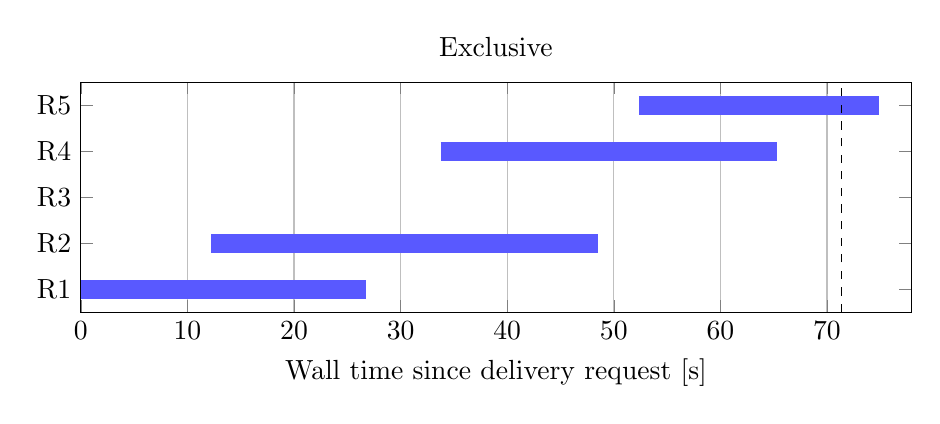
\begin{tikzpicture}
\begin{axis}[width=\linewidth,height=4.5cm,title={Exclusive},xmin=0,xmax=77.894,
ymin=0.5,ymax=5.5,ytick={1,2,3,4,5},yticklabels={R1,R2,R3,R4,R5},xlabel={Wall time since delivery request [s]},xmajorgrids=true]
\addplot+[no marks,line width=7pt,blue!65] coordinates {(0.055,1) (26.755,1)};
\addplot+[no marks,line width=7pt,blue!65] coordinates {(12.254,2) (48.513,2)};
\addplot+[no marks,line width=7pt,blue!65] coordinates {(33.754,4) (65.300,4)};
\addplot+[no marks,line width=7pt,blue!65] coordinates {(52.355,5) (74.898,5)};
\addplot[black,dashed] coordinates {(71.355,0.5) (71.355,5.5)};
\end{axis}
\end{tikzpicture}\par
% region, repetition 4
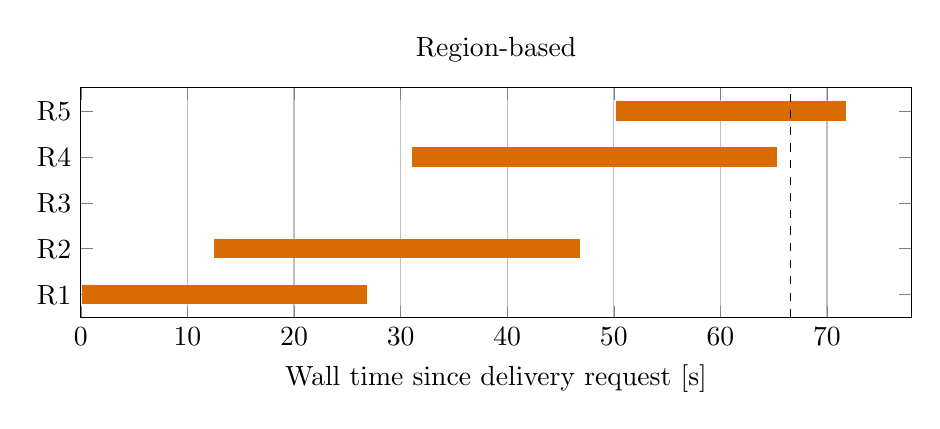
\begin{tikzpicture}
\begin{axis}[width=\linewidth,height=4.5cm,title={Region-based},xmin=0,xmax=77.894,
ymin=0.5,ymax=5.5,ytick={1,2,3,4,5},yticklabels={R1,R2,R3,R4,R5},xlabel={Wall time since delivery request [s]},xmajorgrids=true]
\addplot+[no marks,line width=7pt,orange!85!black] coordinates {(0.078,1) (26.891,1)};
\addplot+[no marks,line width=7pt,orange!85!black] coordinates {(12.478,2) (46.810,2)};
\addplot+[no marks,line width=7pt,orange!85!black] coordinates {(31.078,4) (65.302,4)};
\addplot+[no marks,line width=7pt,orange!85!black] coordinates {(50.178,5) (71.763,5)};
\addplot[black,dashed] coordinates {(66.578,0.5) (66.578,5.5)};
\end{axis}
\end{tikzpicture}\par
\end{document}
